\documentclass{beamer}
\usetheme{default} 

\setbeamercolor{structure}{fg=green!40!black} 
\usebackgroundtemplate{
    \centering
\includegraphics[width=\paperwidth,height=\paperheight]{images/android_wall}
}
\setbeamertemplate{navigation symbols}{}

\usepackage[polish]{babel}
\usepackage[utf8x]{inputenc}
\usepackage{t1enc}
\usepackage{default}
\usepackage{listings}

\lstset{language=java, basicstyle=\small, commentstyle=\color{gray}}
\lstset{frame=single}

\usefoottemplate{
  \vbox{
    \tinycolouredline{structure!25}{
      \color{black}\textbf{
        \insertshortauthor\hfill
        Android @ Szczecin 2011
      } 
    }
%    \tinycolouredline{structure}{
%      \color{white}\textbf{\insertshorttitle}\hfill
%    } 
  }
}

\title{Android @ Szczecin \\ 2011}
\author{Konrad Malawski \\ konrad.malawski@java.pl}

\begin{document}

% 1st steps, basic info about acitivities and views
\documentclass{beamer}
\usetheme{default} 

\setbeamercolor{structure}{fg=Green!50!black} 
\usebackgroundtemplate{
    \centering
\includegraphics[width=\paperwidth,height=\paperheight]{images/android_wall}
}

\usepackage[utf8x]{inputenc}
\usepackage{default}
\usepackage{listings}

\lstset{language=java, basicstyle=\small, commentstyle=\color{gray}}
\lstset{frame=single}

\usefoottemplate{
  \vbox{
    \tinycolouredline{structure!25}{
      \color{white}\textbf{
        \insertshortauthor\hfill
        Android @ Szczecin 2011
      } 
    }
%    \tinycolouredline{structure}{
%      \color{white}\textbf{\insertshorttitle}\hfill
%    } 
  }
}

\title{Android @ Szczecin \\ 2011}
\author{Konrad Malawski \\ konrad.malawski@java.pl}

\begin{document}

\begin{frame}
\titlepage
\end{frame}

\begin{frame}
 \centering
 Konrad Malawski \\
 _\\
 Lunar Logic Polska \\
 PolishJUG \\ 
 GeeCON\\
 KrakówGTUG\\
 _\\
 twitter: @ktosopl\\
 github: ktoso\\
 blog: blog.project13.pl\\
\end{frame}

\begin{frame}
\frametitle{Architektura}

  \begin{figure}[t]
    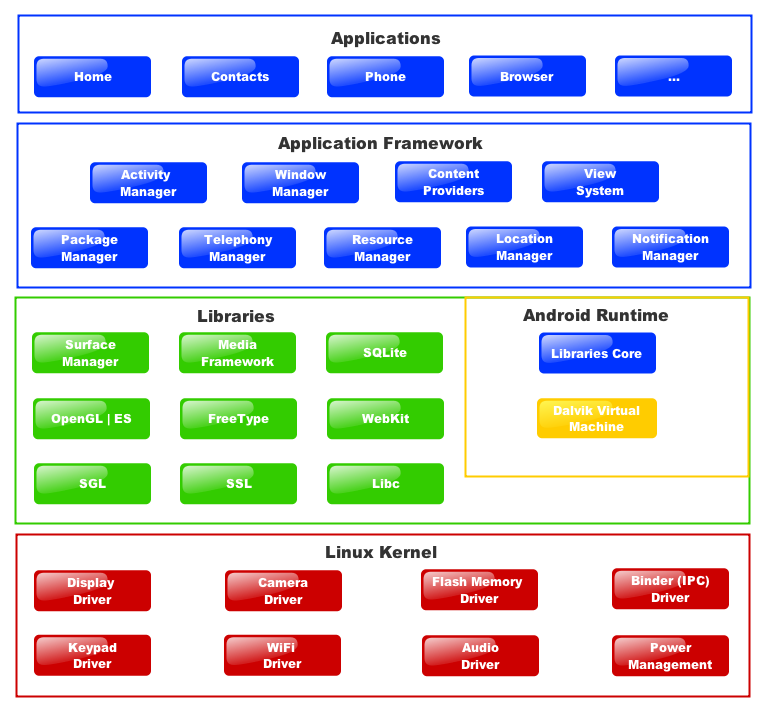
\includegraphics[height=0.62\textheight,keepaspectratio=true,clip=true,trim=0 0 0 100]{images/platform}
    \caption{Architektura systemu Android}
  \end{figure}

\end{frame}


\begin{frame}
\frametitle{It's Linux}
\begin{itemize}
 \item Warto pamiętać, Android = Linux (zawiera glibc etc)
\end{itemize}
\end{frame}

\begin{frame}[fragile]
\frametitle{Activity}
\begin{lstlisting}
  public class MainActivity extends Activity {
    public void onCreate(Bundle savedState) {
      /**/
    }
  }
\end{lstlisting}

\end{frame}


\end{document}


% externalize the name we want to greet into shared properties
% \documentclass{beamer}
% \usetheme{default} 
% 
% \setbeamercolor{structure}{fg=green!40!black} 
% \usebackgroundtemplate{
%     \centering
\includegraphics[width=\paperwidth,height=\paperheight]{images/android_wall}
% }
% \setbeamertemplate{navigation symbols}{}
% 
% \usepackage[polish]{babel}
% \usepackage[utf8x]{inputenc}
% \usepackage{t1enc}
% \usepackage{default}
% \usepackage{listings}
% 
% \lstset{language=java, basicstyle=\small, commentstyle=\color{gray}}
% \lstset{frame=single}
% 
% \usefoottemplate{
%   \vbox{
%     \tinycolouredline{structure!25}{
%       \color{black}\textbf{	
%         \insertshortauthor\hfill
%         Android @ Szczecin 2011
%       } 
%     }
% %    \tinycolouredline{structure}{
% %      \color{white}\textbf{\insertshorttitle}\hfill
% %    } 
%   }
% }
% 
% \title{Android @ Szczecin \\ 2011}
% \author{Konrad Malawski \\ konrad.malawski@java.pl}
% 
% \begin{document}


\begin{frame}
 \begin{center}
  \Huge{Logger}
 \end{center}

\end{frame}



\begin{frame}[fragile]\frametitle{Android Logger}
Logujemy przy pomocy \textbf{android.util.Log}.\\
Korzystamy z niego następująco:

\begin{lstlisting}
class MyClass {
  private final String TAG = getClass()
                             .getSimpleName();

  void doStuff() {
    Log.d(TAG, "doing stuff..."); // debug
  }
}
\end{lstlisting}
\end{frame}

\begin{frame}[fragile]\frametitle{Android Log levels}
Dostępne poziomy logowania to:
\begin{itemize}
 \item \verb|Log.v()| - VERBOSE
 \item \verb|Log.d()| - DEBUG
 \pause \item \verb|Log.i()| - INFO
 \pause \item \verb|Log.w()| - WARN
 \pause \item \verb|Log.e()| - ERROR
 \pause \item \verb|Log.wtf()| \pause - \textbf{W}hat a \textbf{T}errible \textbf{F}ailure
\end{itemize}

\end{frame}

\begin{frame}
 \begin{center}
  \Huge{Data Storage}
 \end{center}

\end{frame}


\begin{frame}\frametitle{Sposoby przechowywania danych}
\begin{itemize}
% http://developer.android.com/guide/topics/data/data-storage.html
 \item  \textbf{Shared Preferences} - Prosty KeyValue store, idealny dla prostych ustawień aplikacji etc
 \pause \item \textbf{Internal Storage} - Zapisywanie plików w swoim formacie na \textbf{wewnątrznej pamięci} urządzenia (dobre dla cache obrazków etc)
 \pause \item \textbf{External Storage} - Zapisywanie plików w swoim formacie na np. \textbf{karcie SD} (dobre dla cache obrazków etc)
 \pause \item \textbf{SQLite Database} - Zwyczajna instancja bazy danych SQLite - m.in. tym sposobem dostajemy informacje o kontaktach
 \pause \item \textbf{Cloud Storage} - Nie trzymamy danych lokalnie, pchamy i pobieramy wszystko z chmurki
\end{itemize}
\end{frame}


\begin{frame}\frametitle{Shared Preferences}
\begin{center}
 \Huge{Shared Preferences} 
\end{center}
\end{frame}

\begin{frame}[fragile]\frametitle{SharedPreferences - API}
Uzyskanie instancji:
\begin{lstlisting}
// zawsze zadziala:
Context ctx = getApplicationContext(); 

// w Activity lub Service jest latwiej:
// ctx = this;

SharedPreferences prefs = PreferenceManager
                 .getDefaultSharedPreferences(ctx);
\end{lstlisting}
\end{frame}


\begin{frame}[fragile]\frametitle{SharedPreferences - Read API}
 Przykład \textbf{odczytania} zmiennej:
\begin{lstlisting}
 // oto jak korzystac z @strings/ w Activity
 String key = getString(R.string.key_sound_notif);

 String s = preferences.getString(key, "undefined");
 
 // analogicznie dla Integer/Long/Double/StringSet
\end{lstlisting}
\end{frame}

\begin{frame}[fragile]\frametitle{SharedPreferences - Write API}
 Przykład \textbf{zapisania} zmiennej:
\begin{lstlisting}
SharedPreferences.Editor editor = preferences.edit();

editor.putString(key, "new value");
// analogicznie dla Integer/StringSet/Double ...

editor.commit();
\end{lstlisting}
\end{frame}


\begin{frame}[fragile]\frametitle{Shared Preferences}
 Shared w sensie ,,wewnątrz \textbf{naszej} aplikacji'', nie między wieloma.\\
 SharedPreferences zapisywane są w: \\
 \begin{center}
  \texttt{/data/data/pl.project13.myapp/shared\_prefs} 
 \end{center}

\pause

Można się tam dobrać gdy się jest \textbf{root}:
\begin{verbatim}
$ abd shell
> cat /data/data/pl.project13.myapp/shared_prefs

<map>
 <string name="pass">zomg_its_plain_text</string>
 <!-- ... -->
</map>
\end{verbatim}
\end{frame}

% SQL kontakty http://developer.android.com/guide/topics/providers/content-providers.html
% todo można by tutaj jeszcze o SQL i poszukiwaniu kontaktów

\begin{frame}\frametitle{Security a SharedPreferences}
\begin{center}
 Wniosek jest prosty:\\ 
 Szyfrujemy ważne rzeczy trzymane gdziekolwiek na komórce.
\end{center}
\end{frame}

\begin{frame}
 \begin{center}
  \Huge{RoboGuice}
 \end{center}

\end{frame}



\begin{frame}\frametitle{Robo Guice - Google Guice for Android}
 \begin{figure}[c]
 
\includegraphics[width=0.5\textwidth]{images/roboguice}  
 \end{figure}
 
 \begin{center}
  Google Guice = \textbf{JSR-330} Dependency Injection for Java
 \end{center}
\end{frame}

\begin{frame}[fragile]\frametitle{RoboGuice - co zyskujemy?}
Przed:
\begin{lstlisting}
class Act extends Activity {
 SharedPreferences prefs;
 EditText mLogin;
 public void onCreate(Bundle savedState) {
  prefs = PreferenceManager
          .getDefaultSharedPreferences(this);
  mLogin = (EditText) findById(R.id.login);
 }
}
\end{lstlisting}

\pause

Po:
\begin{lstlisting}
class Act extends RoboActivity {
 @Inject SharedPreferences prefs;
 @InjectView(R.id.login) EditText mLogin;
 public void onCreate(Bundle savedState){ /**/ }
}
\end{lstlisting}

\end{frame}


\begin{frame}[fragile]\frametitle{Zapięcie RoboGuice w 4 krokach:}
\begin{enumerate}
 \item własny \textbf{App extends RoboApplication} gdzie nadpisujemy \textbf{\#addApplicationModules}
 \pause \item własny \textbf{SzczecinModule extends AbstractAndroidModule}, który dodajemy powyżej
 \pause \item dodanie \verb|<application android:name=".App"| dla naszej aplikacji w \textbf{AndroidManifest.xml}
 \pause \item zamiana \verb|MyActivity extends Activity| na: \verb|MyActivity extends RoboActivity|
\end{enumerate}
\end{frame}


\begin{frame}[fragile]\frametitle{Zadanie: Kroczki do przodu}
\begin{itemize}
 \item podpinamy \textbf{RoboGuice}
 \item zapisujemy \textbf{imię użytkownika} w \textbf{SharedPreferences}
 \item podpinamy \textbf{res/menu/menu.xml} (1 element menu, o nazwie 'settings') (tip: robi się to w \textbf{onCreateOptionsMenu()})
 \item 
\end{itemize} 

tip:
\begin{verbatim}
bindConstant()
.annotatedWith(SharedPreferencesName.class)
.to("pl.project13");
\end{verbatim}
\end{frame}

\begin{frame}
\begin{center}
 \Huge{PreferenceActivity}
\end{center}
\end{frame}

\begin{frame}\frametitle{PreferenceActivity}
\begin{center}
Ręczne edytowanie SharedPreferences szybko robi się nudne...\\
Wtedy właśnie korzystamy z PreferenceActivity:
 \begin{figure}
 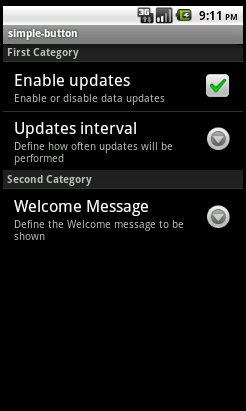
\includegraphics{images/preference_activity}
 \end{figure}
\end{center}
\end{frame}

\begin{frame}[fragile]\frametitle{/res/\textbf{xml/preferences.xml}}
\begin{lstlisting} 
<PreferenceScreen xmlns:android="http://...">
  <PreferenceCategory 
      android:title="Ustawienia Usera"
      android:key="user_preferences">
       
    <CheckBoxPreference 
       android:key="@string/pref_key_notify_user"
       android:summary="Powiadamiaj uzytkownika"
       android:title="Wlacz powiadomienia" 
       android:defaultValue="true"
    />
            
  </PreferenceCategory>
<!-- ... -->
\end{lstlisting}
\end{frame}

\begin{frame}[fragile]\frametitle{/res/\textbf{xml/preferences.xml}}
\begin{lstlisting}
<!-- ... -->
  <PreferenceCategory 
      android:title="Ustawienia pozostale"
      android:key="other_preferences">

    <EditTextPreference
        android:key="@string/pref_key_welcome_msg"
        android:title="Wiadomosc powitalna" 
        android:summary="Wiadomosc jaka zostanie 
                         powitany uzytkownik"
        android:dialogTitle="Wiadomosc powitalna"
        android:dialogMessage="Wpisz wiadomosc:"    
        android:defaultValue="Jak sie masz, " />
  </PreferenceCategory>
</PreferenceScreen>
\end{lstlisting}
\end{frame}

\begin{frame}[fragile]\frametitle{PreferenceActivity - implementacja}
\begin{center}
W przeciwieństwie do powyższych 2 slajdów xml, tutaj kodu jest malutko:
\end{center}
\begin{lstlisting}
public class SettingsActivity 
                       extends PreferenceActivity {

  public void onCreate(Bundle savedInstanceState) {
    super.onCreate(savedInstanceState);

    addPreferencesFromResource(R.xml.preferences);
  }
}
\end{lstlisting}
\end{frame}

\begin{frame}\frametitle{Jak uruchomić inną Activity?}
\begin{center}
I w tym miejscu czas poznać:
\large{Incencje}
\end{center}
\end{frame}

\begin{frame}
\begin{center}
 \Huge{Intent}
\end{center}
\end{frame}

\begin{frame}\frametitle{Intent - czyli ,,Intencja wykonania X''}
Intent'y wykorzystywane są bardzo bardzo intensywnie w androidzie.\\
Poprzez intent działają chociażby:
\begin{itemize}
 \item Otworzenie linka
 \pause \item Wysłanie/odebranie SMSa \pause (Intent albo przez SMSManager)
 \pause \item Uruchomienie usługi (Service)
 \pause \item Uruchomienie Activity
 \pause \item Przekazanie danych innej części aplikacji
 \pause \item nasłuchiwanie na ,,\textbf{system-wide}'' zdarzenia
\end{itemize}
\end{frame}

\begin{frame}[fragile]\frametitle{Intent - czyl ,,Intencja wykonania X''}
\begin{center}
 \textit{Intent = ,,Chciałbym zrobić X''.}

\pause
Chciałbym otworzyć przeglądarkę www:
\end{center}

\begin{lstlisting}
String action = Intent.ACTION_VIEW; 
Uri uri = Uri.parse("http://www.geecon.org")

Intent viewIntent = new Intent(action, uri);
startActivity(viewIntent); // uruchom
\end{lstlisting}
\end{frame}

\begin{frame}[fragile]\frametitle{Intent - przykłady cd.}
\begin{center}
Chcę wysłać SMSa, przy pomocy \textbf{jakiejś aplikacji}, \\
która potrafi się tym zająć.
\end{center}

\begin{lstlisting}
Intent sendIntent = new Intent(Intent.ACTION_VIEW);

sendIntent.putExtra("sms_body", "Halo Szczecin!"); 
sendIntent.setType("vnd.android-dir/mms-sms");

startActivity(sendIntent);
\end{lstlisting}

\pause
SMSy również można wysyłać przy pomocy \textbf{SMSManager}.
\end{frame}

\begin{frame}[fragile]\frametitle{Intent-Filter - ,,Słuchacze''}
Aby ,,słuachć'' na globalne Intent trzeba dodać w \textbf{AndroidManifest.xml}:
\begin{lstlisting}
<application ...>
  <receiver android:name=".SmsReceiver"> 
    <intent-filter> 
      <action android:name=
        "android.provider.Telephony.SMS_RECEIVED" /> 
    </intent-filter> 
  </receiver>
</application>
\end{lstlisting}

\pause

\textbf{MAIN} oraz \textbf{LAUNCHER} dla Activity, definiujące główne Activity naszej aplikacji również rejestrujemy przez Intent-Filtry!

\end{frame}

\begin{frame}[fragile]\frametitle{IntentReciever - przykład dla \textbf{SMS\_RECEIVED}}
\begin{lstlisting}
public class SmsReceiver extends BroadcastReceiver {
  @Override
  public void onReceive(Context context, Intent intent) {
    Bundle bundle = intent.getExtras();
    if(bundle == null) return;

    Object[] pdus = (Object[]) bundle.get("pdus");

    for (Object aPdus : pdus) {
      SmsMessage msg;
      msg = SmsMessage.createFromPdu((byte[]) aPdus);
      
      String from = msg.getOriginatingAddress();
      String body = msg.getMessageBody().toString();
      Log.i(TAG, format(%s: %s, from, body));                     
    }
  }
}
\end{lstlisting}
\end{frame}


\begin{frame}\frametitle{Intent - fun facts}
\begin{itemize}
 \item \textbf{Intent} może być obsłużony przez dowolną aplikację - nie tylko ,,nasze''
 \pause \item W przypadku gdy \textbf{Intent} natrafi 2+ ,,Recievery'', pyta użytkownika którego ma użyć. Przykład: \\
              \pause I: ,,Otwórz ten link.''\\
              \pause A: ,,W Operze czy w Firefoxie?''
              
             
 \pause \item \textbf{Intent} może nieść ze sobą masę dodatkowych informacji oraz flag. Vide metody klasy Intent.
\end{itemize}
\end{frame}










% \end{document}


% more fun with views
\documentclass{beamer}
\usetheme{default} 

\setbeamercolor{structure}{fg=green!40!black} 
\usebackgroundtemplate{
    \centering
\includegraphics[width=\paperwidth,height=\paperheight]{images/android_wall}
}
\setbeamertemplate{navigation symbols}{}

\usepackage[polish]{babel}
\usepackage[utf8x]{inputenc}
\usepackage{t1enc}
\usepackage{default}
\usepackage{listings}

\lstset{language=java, basicstyle=\small, commentstyle=\color{gray}}
\lstset{frame=single}

\usefoottemplate{
  \vbox{
    \tinycolouredline{structure!25}{
      \color{black}\textbf{	
        \insertshortauthor\hfill
        Android @ Szczecin 2011
      } 
    }
%    \tinycolouredline{structure}{
%      \color{white}\textbf{\insertshorttitle}\hfill
%    } 
  }
}

\title{Android @ Szczecin \\ 2011}
\author{Konrad Malawski \\ konrad.malawski@java.pl}

\begin{document}




\begin{frame}
 \begin{center}
  \Huge{Moar* Fun with Views}
 \end{center}
\begin{flushright}
* sic
\end{flushright}
\end{frame}


\begin{frame}\frametitle{Zmierzamy w kierunku kolejnego Activity}
\begin{itemize}
 \item Dodamy nowe Activity
 \pause \item Będzie pobierać coś z sieci (lub udawać) oraz
 \pause \item hint: przyda się jakiś progress bar etc
 \pause \item utworzy z tych danych ListView
 \pause \item przejdziemy do niego przez \textbf{menu} w obecnym Activity
\end{itemize}
\end{frame}

% Menus
\begin{frame}
\begin{center}
 \Huge{Menu}
\end{center}
\end{frame}


\begin{frame}\frametitle{Menu (vide przycisk menu)}
\begin{center}
 Cel:\\
 \begin{figure}
  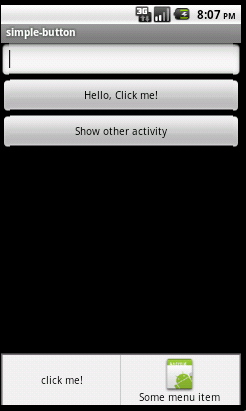
\includegraphics[height=.75\textheight]{images/sample_with_menu}
 \end{figure}
\end{center}
\end{frame}

\begin{frame}[fragile]\frametitle{res/menu/sample\_menu.xml}
\begin{lstlisting}
<menu xmlns:android="http://...">

    <item android:id="@+id/click_me_menu_item"
          android:title="click me!"
            />

    <item android:id="@+id/some_menu_item"
          android:title="Some menu item"
          android:icon="@drawable/icon"
            />
</menu>
\end{lstlisting}
\end{frame}

\begin{frame}[fragile]\frametitle{SomeActivity\#onCreateOptionsMenu}
\begin{lstlisting}
@Override
public boolean onCreateOptionsMenu(Menu menu) { 
  MenuInflater inflater = getMenuInflater();

  inflater.inflate(R.menu.sample_menu, menu);
  return true;
}
\end{lstlisting}
\end{frame}

\begin{frame}[fragile]\frametitle{SomeActivity\#onCreateOptionsMenu}
\begin{lstlisting}
@Override
public boolean onCreateOptionsMenu(Menu menu) { 
  MenuInflater inflater = getMenuInflater();

  inflater.inflate(R.menu.sample_menu, menu);
  return true; // true == ma zostac pokazane
}
\end{lstlisting}
\end{frame}

\begin{frame}[fragile]\frametitle{SomeActivity\#onOptionsItemSelected}
\begin{lstlisting}
@Override
public boolean onOptionsItemSelected(MenuItem item) {
  int itemId = item.getItemId();

  switch (itemId){
    case R.id.click_me_menu_item:
      doSomething();
      break;
    default:
      Log.i(TAG, "Some weird action was requested");
  }

  return true; 
}
\end{lstlisting}
\end{frame}

\begin{frame}[fragile]\frametitle{SomeActivity\#onOptionsItemSelected}
\begin{lstlisting}
@Override
public boolean onOptionsItemSelected(MenuItem item) {
  int itemId = item.getItemId();

  switch (itemId){
    case R.id.click_me_menu_item:
      doSomething();
      break;
    default:
      Log.i(TAG, "Some weird action was requested");
      return false;
  }

  return true; // true == obsluzylismy event
               //      == no need to bubble it
}
\end{lstlisting}
\end{frame}


% MORE FUN UI STUFF
\begin{frame}
\begin{center}
 \Huge{Giving Feedback} \\
 \large{(Toasts and Dialogs)}
\end{center}
\end{frame}


\begin{frame}[fragile]\frametitle{Pyszne tosty z masełkiem (android.widget.Toast)}

\begin{figure}[h]
 \centering
 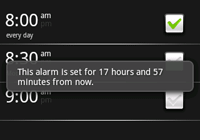
\includegraphics[height=0.40\textheight,keepaspectratio=true]{images/toast}
\end{figure}

 Przykład użycia: 
 \begin{lstlisting}
Toast.makeText(getApplicationContext(),
               "Halo Szczecin!", 
               Toast.LENGTH_LONG)
     .show();
 \end{lstlisting}

\end{frame}

\begin{frame}[fragile]
\frametitle{Co więcej potrafi Toast?}
\begin{lstlisting}
 Toast t = Toast.makeText(this, txt, LENGTH_SHORT);
\end{lstlisting}

\pause

Można mu zmienić pozycję:
\begin{lstlisting}
t.setGravity(Gravity.TOP|Gravity.LEFT, 0, 0);
\end{lstlisting}

\pause

lub podmienić widok:
\begin{lstlisting}
View customView = findViewById(R.id.custom_view);
/**/
t.setView(customView)
 \end{lstlisting}

\end{frame}

\begin{frame}
 \begin{center}
  \Huge{Dialog}
 \end{center}
\end{frame}


\begin{frame}\frametitle{Dialog - wyskakuje 'nad' Activity}
\begin{columns}
 \column{.5\textwidth}
  \begin{figure}
   \centering
   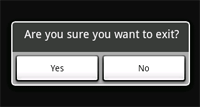
\includegraphics[width=.7\textwidth]{images/dialog_buttons}
  \end{figure}
  \begin{figure}
   \centering
   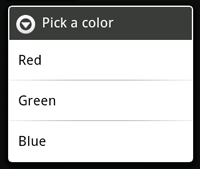
\includegraphics[width=.7\textwidth]{images/dialog_list}
  \end{figure}
 \column{.5\textwidth}
 \begin{figure}
   \centering
   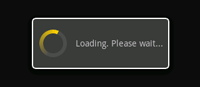
\includegraphics[width=.7\textwidth]{images/dialog_progress_spinning}
  \end{figure}
  \begin{figure}
   \centering
   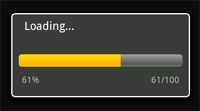
\includegraphics[width=.7\textwidth]{images/dialog_progress_bar}
  \end{figure}
\end{columns}
\end{frame}

% \begin{frame}[fragile]\frametitle{List Dialog}
% \begin{lstlisting}
% final CharSequence[] items = {"Red", "Green", "Blue"};
% 
% AlertDialog.Builder builder = new AlertDialog.Builder(this);
% builder.setTitle("Pick a color");
% builder.setItems(items, new DialogInterface.OnClickListener() {
%  public void onClick(DialogInterface dialog, int item) {
%   Toast.makeText(getApplicationContext(), items[item], Toast.LENGTH_SHORT).show();
%  }
% });
% AlertDialog alert = builder.create();
% \end{lstlisting}
% \end{frame}

\begin{frame}[fragile]\frametitle{Progress Dialog (Spinning)}
\begin{lstlisting}
ProgressDialog dialog = ProgressDialog
                           .show(MyActivity.this, 
                                 "", 
                                 "Loading. Please wait...", 
                                 true);
\end{lstlisting}

\begin{figure}
 \centering
 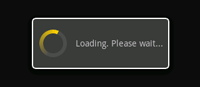
\includegraphics[width=.5\textwidth]{images/dialog_progress_spinning}
\end{figure}

\pause

\begin{lstlisting}
dialog.hide();
\end{lstlisting}
\end{frame}

\begin{frame}[fragile]\frametitle{Super Fast Java Reminder - \textbf{this}}
Pamiętamy dlaczego w poprzednim przykładzie powinno (często) być \textbf{MyActivity.this}?
\begin{lstlisting}
class Outer extends Activity { 

  void onCreate(Bundle savedState) {

    new OnClickListener() {
      public void onClick(View view) {
        new Intent(this, /*...*/); // ZLE!
      }
    }

  }
}
\end{lstlisting}
\end{frame}

\begin{frame}[fragile]\frametitle{Super Fast Java Reminder - \textbf{this}}
Oto jak dobrać się do ,,zewnętrznego'' \textbf{this}:
\begin{lstlisting}
class Outer extends Activity { 

  void onCreate(Bundle savedState) {

    new OnClickListener() {
      public void onClick(View view) {
        new Intent(Outer.this, /*...*/); // Dobrze
      }
    }

  }
}
\end{lstlisting}
\end{frame}







\end{document}


% more fun with views
\documentclass{beamer}
\usetheme{default} 

\setbeamercolor{structure}{fg=green!40!black} 
\usebackgroundtemplate{
    \centering
\includegraphics[width=\paperwidth,height=\paperheight]{images/android_wall}
}
\setbeamertemplate{navigation symbols}{}

\usepackage[polish]{babel}
\usepackage[utf8x]{inputenc}
\usepackage{t1enc}
\usepackage{default}
\usepackage{listings}

\lstset{language=java, basicstyle=\small, commentstyle=\color{gray}}
\lstset{frame=single}

\usefoottemplate{
  \vbox{
    \tinycolouredline{structure!25}{
      \color{black}\textbf{	
        \insertshortauthor\hfill
        Android @ Szczecin 2011
      } 
    }
%    \tinycolouredline{structure}{
%      \color{white}\textbf{\insertshorttitle}\hfill
%    } 
  }
}

\title{Android @ Szczecin \\ 2011}
\author{Konrad Malawski \\ konrad.malawski@java.pl}

\begin{document}


\begin{frame}
 \begin{center}
  \Huge{AppWidgets}
 \end{center}
\end{frame}

\begin{frame}\frametitle{AppWidget}
\begin{itemize}
 \item Good news: Bardzo proste!
 \item AppWidget = specjalny BroadcastReciever
 \item a rozmiar etc, deklarujemy w \textbf{res/xml/my\_widget.xml}
\end{itemize}
\end{frame}


\begin{frame}[fragile]\frametitle{AppWidgetProvider}
\textbf{AppWidgetProvider}, musi zostać zarejestrowany w \textbf{AndroidManifest.xml} (w <application/>):
\begin{lstlisting}
<receiver android:name=".ui.appwidgets.MyWidgetProvider">
  <intent-filter>
    <action android:name="android.appwidget.action.APPWIDGET_UPDATE"/>
  </intent-filter>
  <meta-data android:name="android.appwidget.provider"
             android:resource="@xml/my_widget"/>
</receiver>
\end{lstlisting}
\end{frame}

\begin{frame}[fragile]\frametitle{res/xml/\textbf{my\_widget.xml}}
\begin{lstlisting}
<appwidget-provider xmlns:android="http://schemas.android.com/apk/res/android"
    android:minWidth="294dp"
    android:minHeight="72dp"
    android:updatePeriodMillis="86400000"
    android:previewImage="@drawable/preview_widget"
    android:initialLayout="@layout/widget">
</appwidget-provider>
\end{lstlisting}
Deklarowanie tego w XML jest wygodniejsze - mamy filtrowanie folderów (-v11).
\end{frame}



\begin{frame}[fragile]\frametitle{AppWidget - implementacja}
\begin{lstlisting}
public class MyWidgetProvider extends AppWidgetProvider {

  @Override
  public void onUpdate(Context context, 
                       AppWidgetManager appWidgetManager, 
                       int[] appWidgetIds) {

    // Provider obsluguje WIELE (N) widzetow!
    final int N = appWidgetIds.length;

    // aktualizujemy kazgego
    for (int i = 0; i < N; i++) {
      int appWidgetId = appWidgetIds[i];
      populateView(context, appWidgetManager, 
                            appWidgetId);
    }
  }
\end{lstlisting}
\end{frame}

\begin{frame}[fragile]\frametitle{AppWidget - implementacja}
\begin{lstlisting}
private void populateView(Context context, AppWidgetManager appWidgetManager, int appWidgetId) {
  // Przygotowujemy intent do odpalenia "on click"
  Intent intent = new Intent(context, ViewDetailsActivity.class);
  PendingIntent pendingIntent = PendingIntent.getActivity(context, 0, intent, 0);

  // rejestrujemy onClickListener'a troszke inaczej:
  RemoteViews views = new RemoteViews(context.getPackageName(), R.layout.widget);
  views.setOnClickPendingIntent(R.id.container, pendingIntent);
 
  // aktualizujemy widok widzetu (prosimy menagera o to)
  appWidgetManager.updateAppWidget(appWidgetId, views);
}
} // end of class
\end{lstlisting}
\end{frame}



\begin{frame}
\begin{center}
\Huge{Notifications}
\end{center}
\end{frame}

\begin{frame}\frametitle{Notificaion - przykład}
\begin{figure}
 \centering
 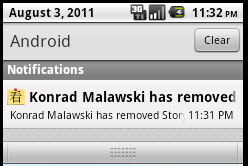
\includegraphics[width=0.7\textwidth]{images/notification_android_2_2}
\end{figure}
\end{frame}


\begin{frame}[fragile]\frametitle{NorificationManager}
\begin{lstlisting}
class MyActivity extends RoboActivity {
  
  @Inject
  NotificationManager notificationManager;

}
\end{lstlisting}
\pause Albo oczywiście \textbf{Service}.
\end{frame}


\begin{frame}[fragile]\frametitle{NorificationManager - 1/3}
\begin{lstlisting}
int icon = R.drawable.ic_kanbanery;
long when = System.currentTimeMillis();

Notification notification = new Notification(icon, title, when);

// ...
\end{lstlisting}
\end{frame}


\begin{frame}[fragile]\frametitle{NorificationManager - 2/3}
\begin{lstlisting}
int icon = R.drawable.ic_kanbanery;
long when = System.currentTimeMillis();

Notification notification = new Notification(icon, title, when);

Intent notificationIntent = new Intent(this, ColumnsActivity.class);
PendingIntent onClickIntent = PendingIntent.getActivity(this, 0, notificationIntent, 0);

// ...
\end{lstlisting}
\end{frame}

\begin{frame}[fragile]\frametitle{NotificationManager - 3/3}
\begin{lstlisting}
int icon = R.drawable.ic_kanbanery;
long when = System.currentTimeMillis();

Notification notification = 
                 new Notification(icon, title, when);

Intent notificationIntent = new Intent(this, 
                              ColumnsActivity.class);
PendingIntent contentIntent = PendingIntent
        .getActivity(this, 0, notificationIntent, 0);

notification.setLatestEventInfo(context, title, 
                                msg, contentIntent);
notification.flags = Notification.FLAG_AUTO_CANCEL;


notificationManager.notify(ACTION_ID, // explain 
                           notification);
\end{lstlisting}
\end{frame}






\end{document}



% final task about maps and sms
% ------------------------------ MAPS ------------------------------ 
\begin{frame}\frametitle{Google Maps}

\begin{figure}[tc]
  \centering
  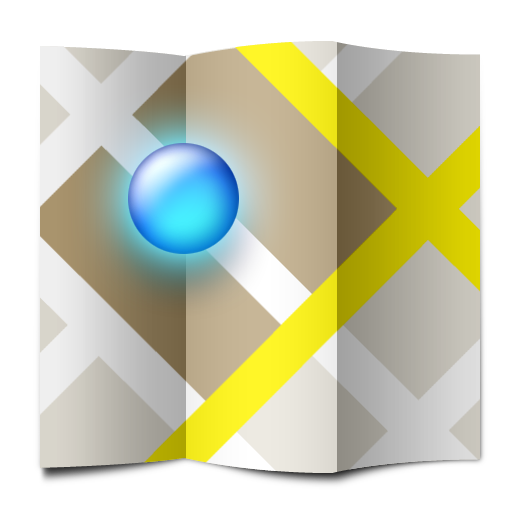
\includegraphics[height=0.45\textheight,keepaspectratio=true]{images/maps_icon}
\end{figure}

Istnieje pewien ''problem'' z Google Maps oraz niektórymi innymi API. \\
\textbf{Nie są one dostępne bez odpowiedniego klucza oraz podpisania swojej aplikacji!}
\end{frame}


\begin{frame}\frametitle{MapsAPI key sign-up}
\begin{center}
  Rejestrujemy są po klucz na: \\
  http://code.google.com/intl/pl-PL/android/maps-api-signup.html \\
  BitLy: \textbf{http://bit.ly/mapsapiandroid}
\end{center}
\end{frame}


\begin{frame}[fragile]\frametitle{Zdobywanie MD5 klucza 'debug'}
\begin{lstlisting}
 keytool -list -alias androiddebugkey \
-keystore <path_to_debug_keystore>.keystore \
-storepass android -keypass android
\end{lstlisting}
\end{frame}


\begin{frame}[fragile]\frametitle{Zdobywanie Md5 klucza 'release'}

\textbf{keytool -list -keystore ~/android.keystore }

\begin{lstlisting}
Keystore type: JKS
Keystore provider: SUN

Your keystore contains 1 entry
android-key, Jul 3, 2011, PrivateKeyEntry, 
Certificate fingerprint (MD5): AA:AA:AA:AA...
\end{lstlisting}

\end{frame}


\begin{frame}\frametitle{Oto co dostaniemy:}
\begin{figure}
 \centering
 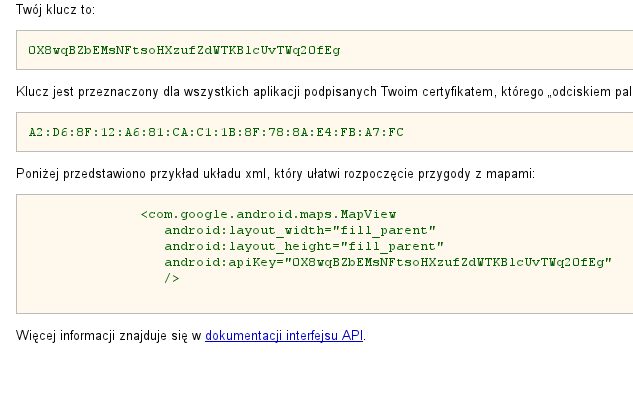
\includegraphics[width=\textwidth,keepaspectratio=true]{images/maps_get_key}
\end{figure} 
\end{frame}


\begin{frame}[fragile]\frametitle{Permissions}

W tym przypadku interesują następujące \verb|<uses-permission/>|:

\begin{itemize}
 \item \verb|android.permission.ACCESS_COARSE_LOCATION|
 \item \verb|android.permission.ACCESS_FINE_LOCATION|
\end{itemize}

oraz (skoro chcemy wyświetlić mapkę)
\begin{itemize}
 \item \verb|android.permission.INTERNET|
\end{itemize}

\pause
Dodatkowo jeszcze deklarujemy wykorzystanie biblioteki maps:
\begin{verbatim}
 <uses-library android:name="com.google.android.maps" />
\end{verbatim}

\textbf{Uwaga!}
\begin{lstlisting}
<application>
  <uses-library/> 
</application>
<uses-permission/>
\end{lstlisting}
\end{frame}

\begin{frame}\frametitle{Co na pewno się przyda?}
\begin{itemize}
 \item \textbf{LocationManager}
 \item \textbf{MapView}
 \item bardzo wygodny jest \textbf{MapActivity}
 \item tip: dostępny jest \textbf{GPS} i \textbf{NETWORK} location provider
\end{itemize}
\end{frame}
 
\begin{frame}[fragile]\frametitle{Zadanie: Google Maps App}
\begin{itemize}
 \item mapka, wycentrowana na obecnym położeniu telefonu
 \item podczas odświeżenia lokalizacji ma pojawiać się Toast z nową lokalizacją (oraz recentrujemy mapkę)
 \item obecne położenie ma być zaznaczone markerem: \textbf{http://bit.ly/gmapmark}
 \item w przypadku oddalenia się od miejsca X (dowolne) należy odpalić '\textbf{alarm}'
 \item wyślij sobie sms gdy przyjdziesz do domu, \textit{,,Home, Sweet Home!''}
 \item zaskocz nas czymś!
\end{itemize}
\end{frame}


 

\end{document}
